\documentclass[t,11pt,compress,xcolor=table,hyperref={bookmarks=false}]{beamer}
\usepackage{textcomp}
\usepackage{amsmath}

\usepackage[makeroom]{cancel}

\usepackage{amssymb}
\usepackage{mathrsfs}
\usepackage{graphicx}
\usepackage{colortbl}
\usepackage[table]{xcolor}
\usepackage{geometry}
\usepackage{beamerthemeshadow}
\usepackage{enumerate}
\usepackage{tikz}
\usepackage{tabu}
\usepackage{esint}
\usepackage{slashed}
\usepackage{pifont}
\usetikzlibrary{arrows}

%\usepackage{epstopdf}
%\epstopdfsetup{update}

\definecolor{DarkGreen}{RGB}{18,173,42}
\definecolor{DarkRed}{RGB}{202,0,42}

\renewcommand{\d}{\textrm{d}}
\newcommand{\e}{\textrm{e}}

\mode<presentation>{
 \usetheme{Antibes}
 \setbeamercovered{transparent}
}


\title[]{\textbf{\textsf{Fire Emergencies in Seattle}}}

\vspace{-0.7cm}
\author[]{
\textsf{\large\textbf{Correlations with Human Activity and Rain Patterns}}
\\
\textsf{}
\\
\textsf{}
\\
\textsf{\large\textbf{Sergio C. Vargas}} 
}

\institute{}
\date{}


\begin{document}

\begin{frame}[plain]
\titlepage
\vspace{-2.2 cm}
\begin{center}
\textsf{\small{supervised by}}
\\
\textsf{\large\textbf{Srdjan Santic}}
\end{center}
\vspace{-0.5 cm}
\begin{figure}
\centering

\includegraphics[height=2cm]{figs/sp_logo}
\end{figure}
\vspace{-1 cm}
\begin{center}
\textsf{\large{\textbf{Springboard}}}
\\
\textsf{\small{Oct 18, 2018}}
\end{center}
\end{frame}


\begin{frame}{Motivation}

\begin{center}
\large
Can we identify trends in 911 fire calls in Seattle?
\\
Can we find patterns, or correlate them with factors such as rain patterns?
\end{center}
\vspace{-0.4cm}
\begin{figure}[ht!]
\centering
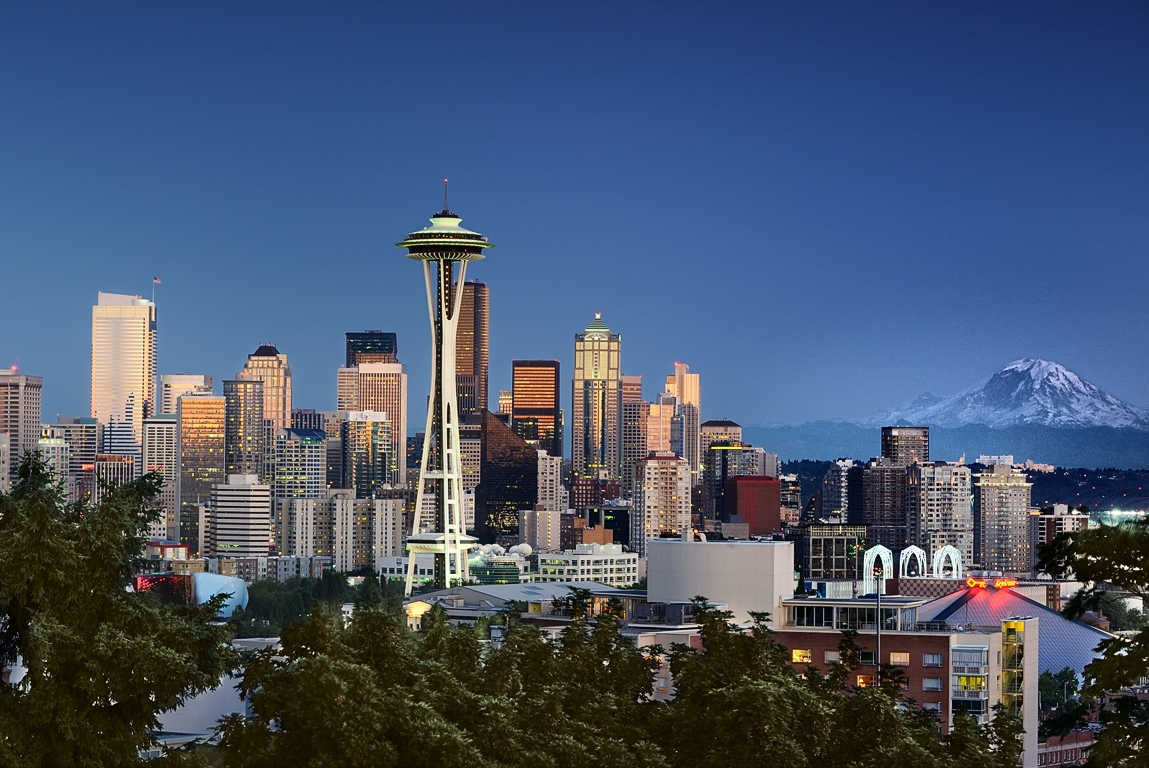
\includegraphics[scale=0.22]{figs/Seattle_Pic.jpg}
%\caption{ }
\label{pic}
\end{figure}
\vspace{-0.7cm}
\begin{center}
{\tiny License notice: \href{https://www.flickr.com/people/43518209@N00}{Bala} from Seattle, USA, \href{https://commons.wikimedia.org/wiki/File:Seattle_from_Kerry_Park_(1).jpg}{Seattle from Kerry Park (1)}, \href{https://creativecommons.org/licenses/by/2.0/legalcode}{CC BY 2.0}.}
\end{center}


\end{frame}


\begin{frame}
\frametitle{Outline}
\tableofcontents
\end{frame}




\section{Sources and Data Sets}


\begin{frame}{Sources and Data Sets}
\vspace{0.3cm}
\begin{itemize}
\Large
\item Seattle Monthly Rain Gauge Accumulations \cite{Daniels2018}
\item Seattle Fire 911 Calls in 2010 and 2011 \cite{FireData2018}
\item Washington State Holidays in 2010 and 2011 \cite{OfficeHolidays2010,OfficeHolidays2011}
\end{itemize}
\end{frame}



\begin{frame}{Sources and Data Sets}
\begin{itemize}
\item {\Large Seattle Monthly Rain Gauge Accumulations \cite{Daniels2018}}
\end{itemize}
\vspace{-0.6cm}
\begin{figure}[ht!]
\centering
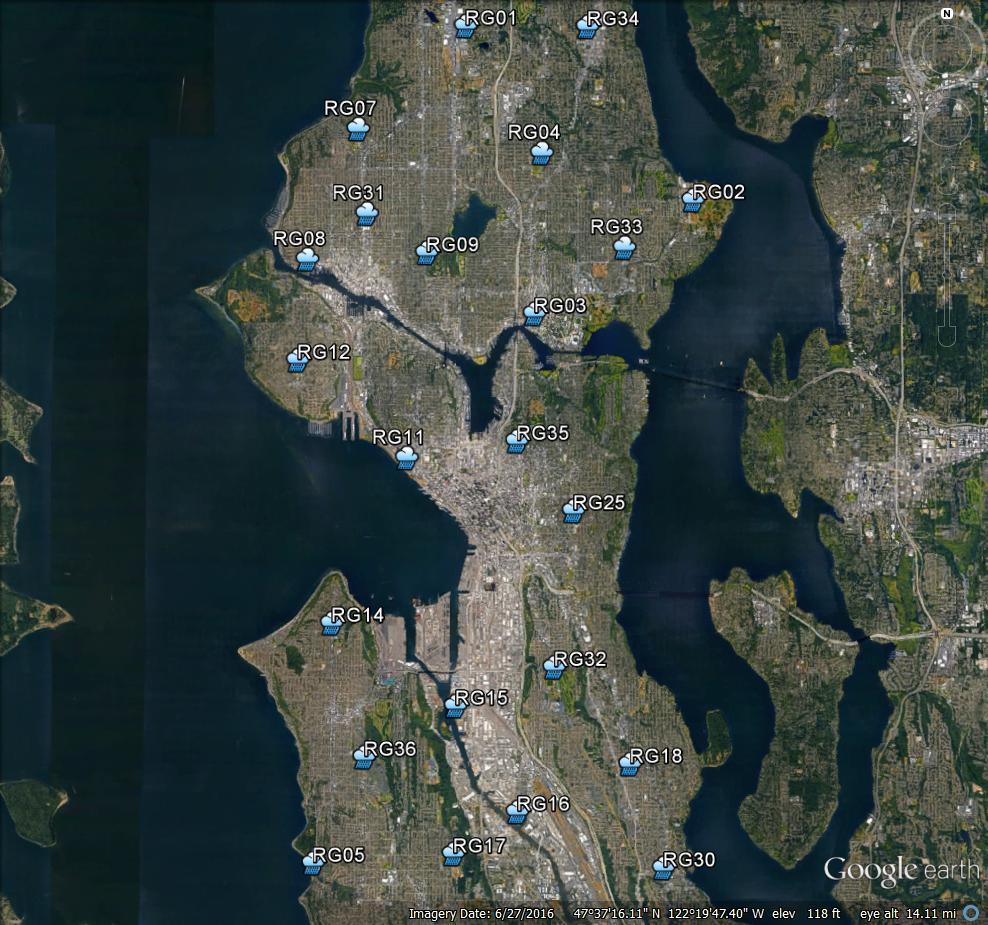
\includegraphics[scale=0.18]{figs/SPU_DWW_RGs.jpg}
\end{figure}
\end{frame}


\begin{frame}{Sources and Data Sets}
\begin{itemize}
\item {\Large Seattle Fire 911 Calls in 2010 and 2011 \cite{FireData2018}}
\end{itemize}
\vspace{-0.3cm}
\begin{figure}[ht!]
\centering
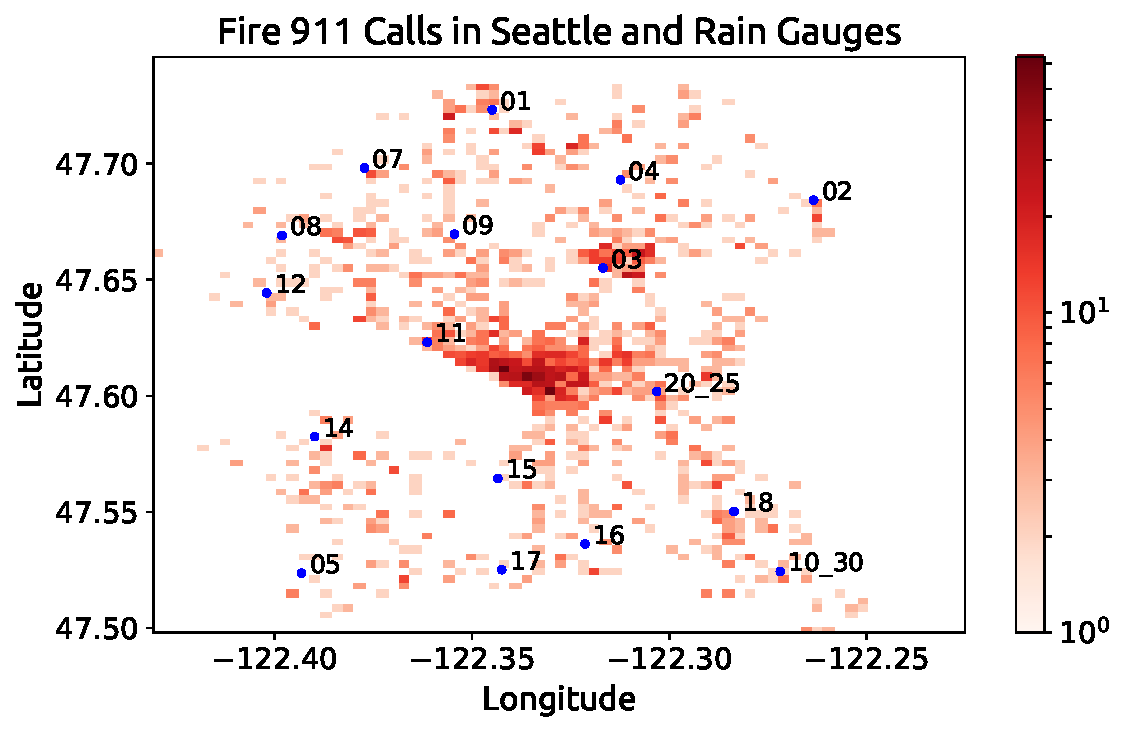
\includegraphics[scale=0.52]{figs/2DHist.pdf}
\end{figure}
\end{frame}

\begin{frame}{Sources and Data Sets}
\begin{itemize}
\item {\Large Washington State Holidays in 2010 and 2011 \cite{OfficeHolidays2010,OfficeHolidays2011}}
\end{itemize}
\vspace{0.3cm}
\begin{center}
\Large
Holidays and Weekends accounted for
\\
31.6\% of 2010 and 2011.
\\
\vspace{0.3cm}
Are there more fires on off days?
\end{center}
\end{frame}


\section{EDA Findings and Analysis}

\begin{frame}{EDA Findings and Analysis: Rain and Fire}
\begin{figure}[ht!]
\centering
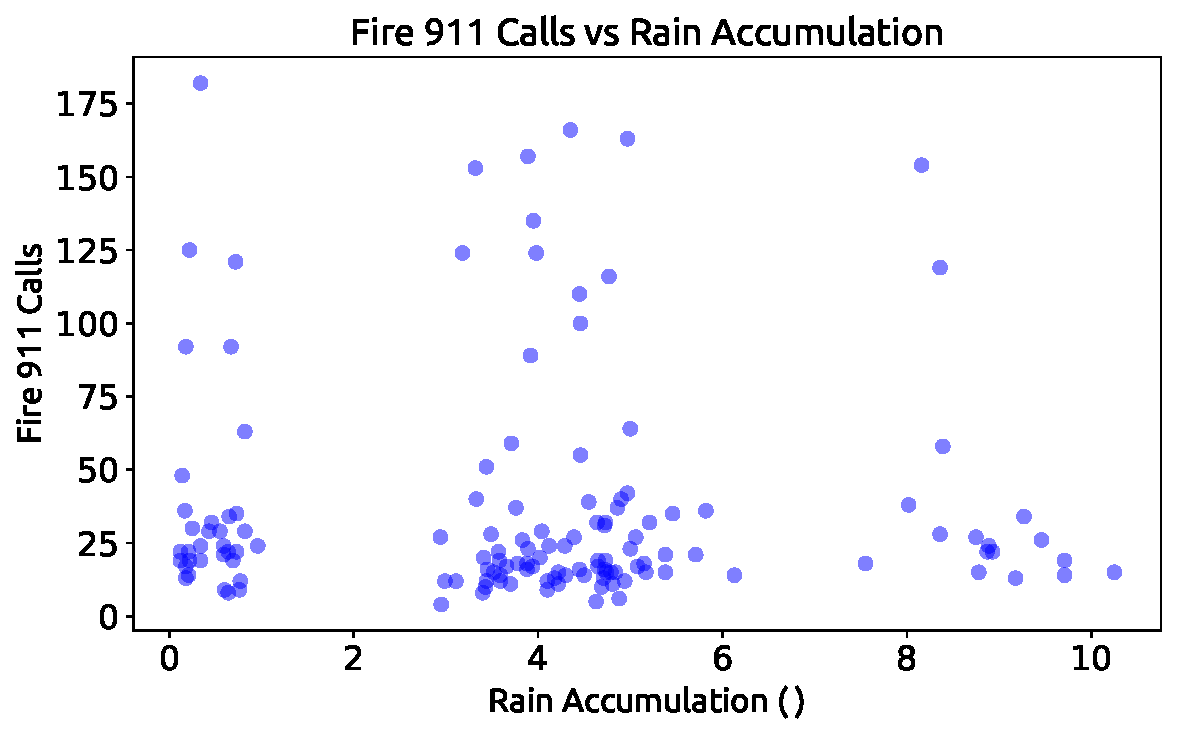
\includegraphics[scale=0.5]{figs/NoCor.pdf}
\end{figure}
\end{frame}

\begin{frame}{EDA Findings and Analysis: Time of the Day and Fire}
\begin{figure}[ht!]
\centering
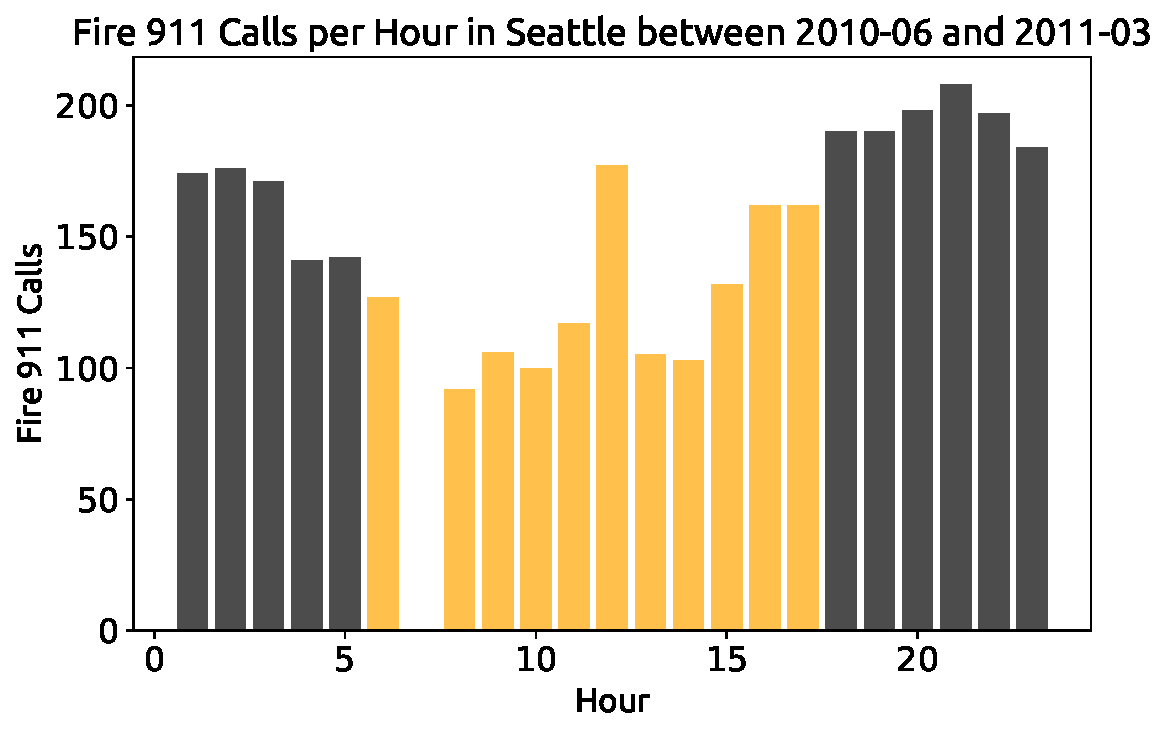
\includegraphics[scale=0.5]{figs/TimeOfTheDay.pdf}
\end{figure}
\end{frame}

\section{Machine Learning Analysis}

\begin{frame}[fragile]{Implemented Clusterings}

\begin{itemize}
\item Only on \verb|Longitude| and \verb|Latitude|: \verb|MinMaxScaler| + \verb|KMeans|.

\item \verb|PCA| dimensional reduction with and without previously scaling with \verb|StandardScaler|. \verb|MinMaxScaler| + \verb|KMeans| on the projected 2D and 3D data.

\item All data without PCA: \verb|MinMaxScaler| + \verb|KMeans|.
\end{itemize}

We decide the ideal $k$ using inertia, silhouette, gap statistic and the gap criterium of Tibshirani, Walther, Hastie, 2002 \cite{Tibshirani}.

\end{frame}

\subsection{Clustering Location only}

\begin{frame}{Sectorizing the City}
\begin{figure}[ht!]
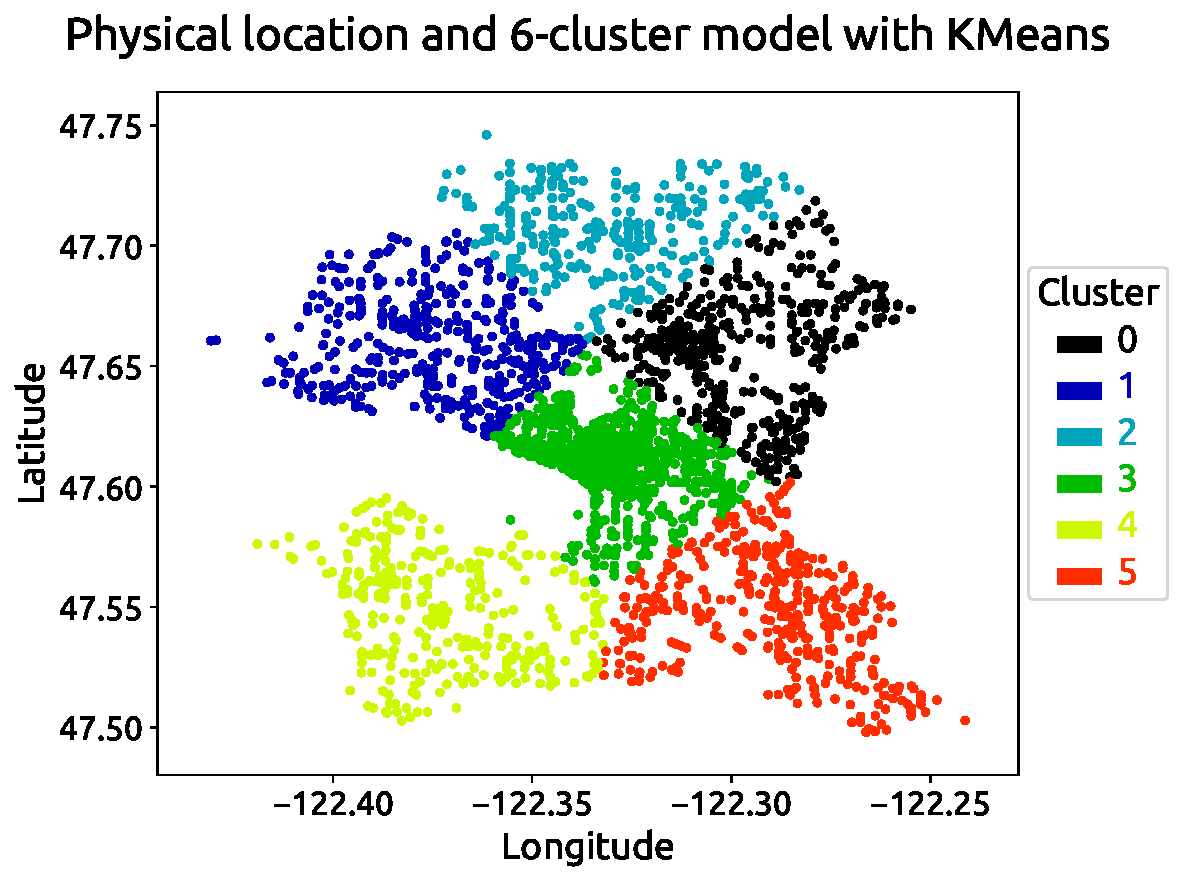
\includegraphics[scale=0.45]{figs/STORY_loc_location.pdf}
\end{figure}
\end{frame}

\begin{frame}{Inertia and average silhouette}
\begin{figure}
\hspace*{-0.9cm}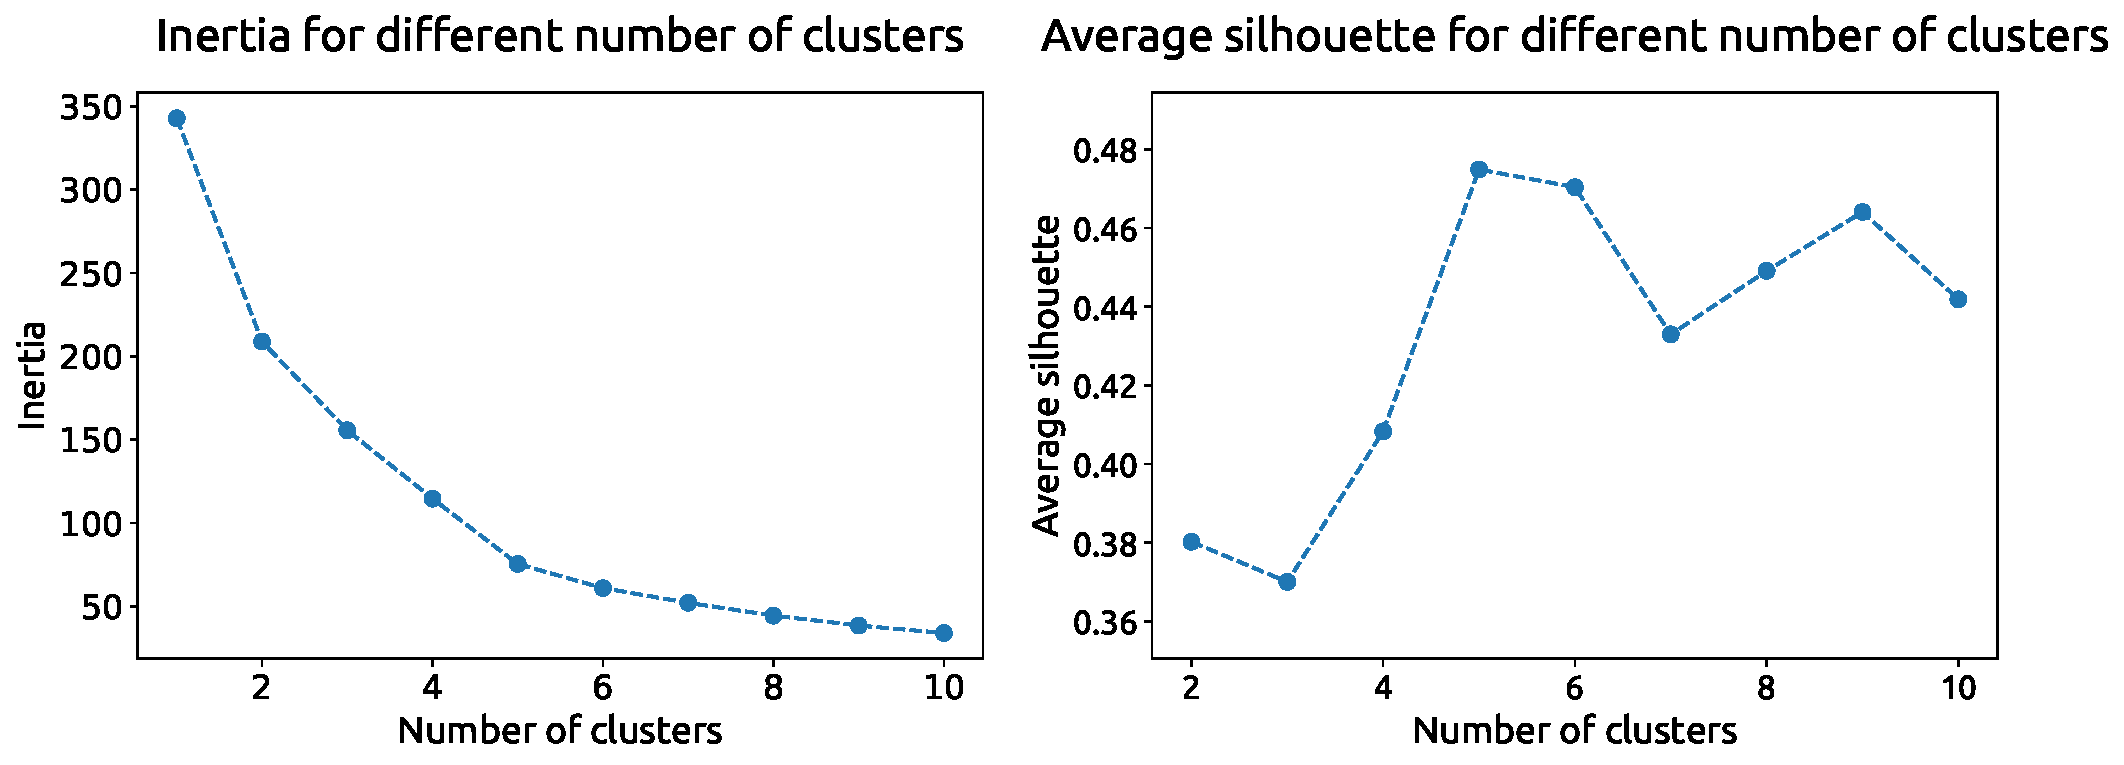
\includegraphics[scale=0.35]{figs/loc_parfigs_1.pdf}
\end{figure}
 \end{frame}

\begin{frame}{Gap and Gap criterium}
\begin{figure}
\hspace*{-0.9cm}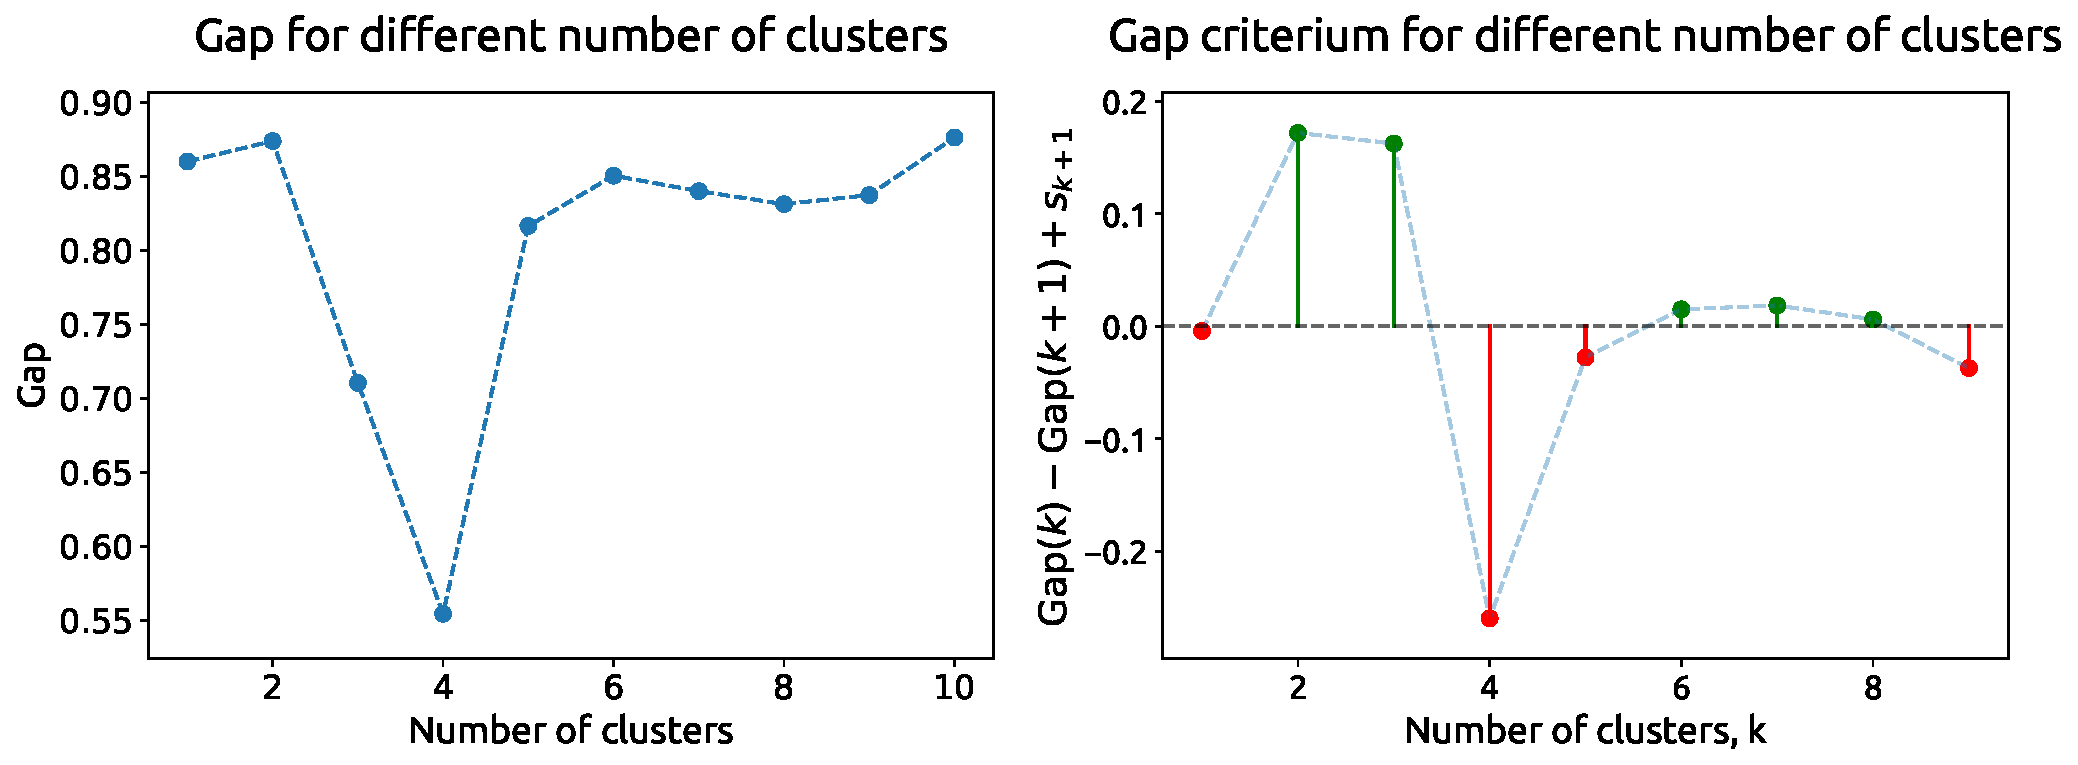
\includegraphics[scale=0.35]{figs/loc_parfigs_2.pdf}
\end{figure}
From \cite{Tibshirani}: Best $k$ is the lowest one that satisfies	
\begin{equation}\label{eq_gap_crit}
\mathrm{Gap}(k) - \mathrm{Gap}(k+1) + s_{k+1} \geq 0 \, .
\end{equation}
\end{frame}


\begin{frame}{Silhouette Plot}
\begin{figure}
\hspace*{-0.9cm}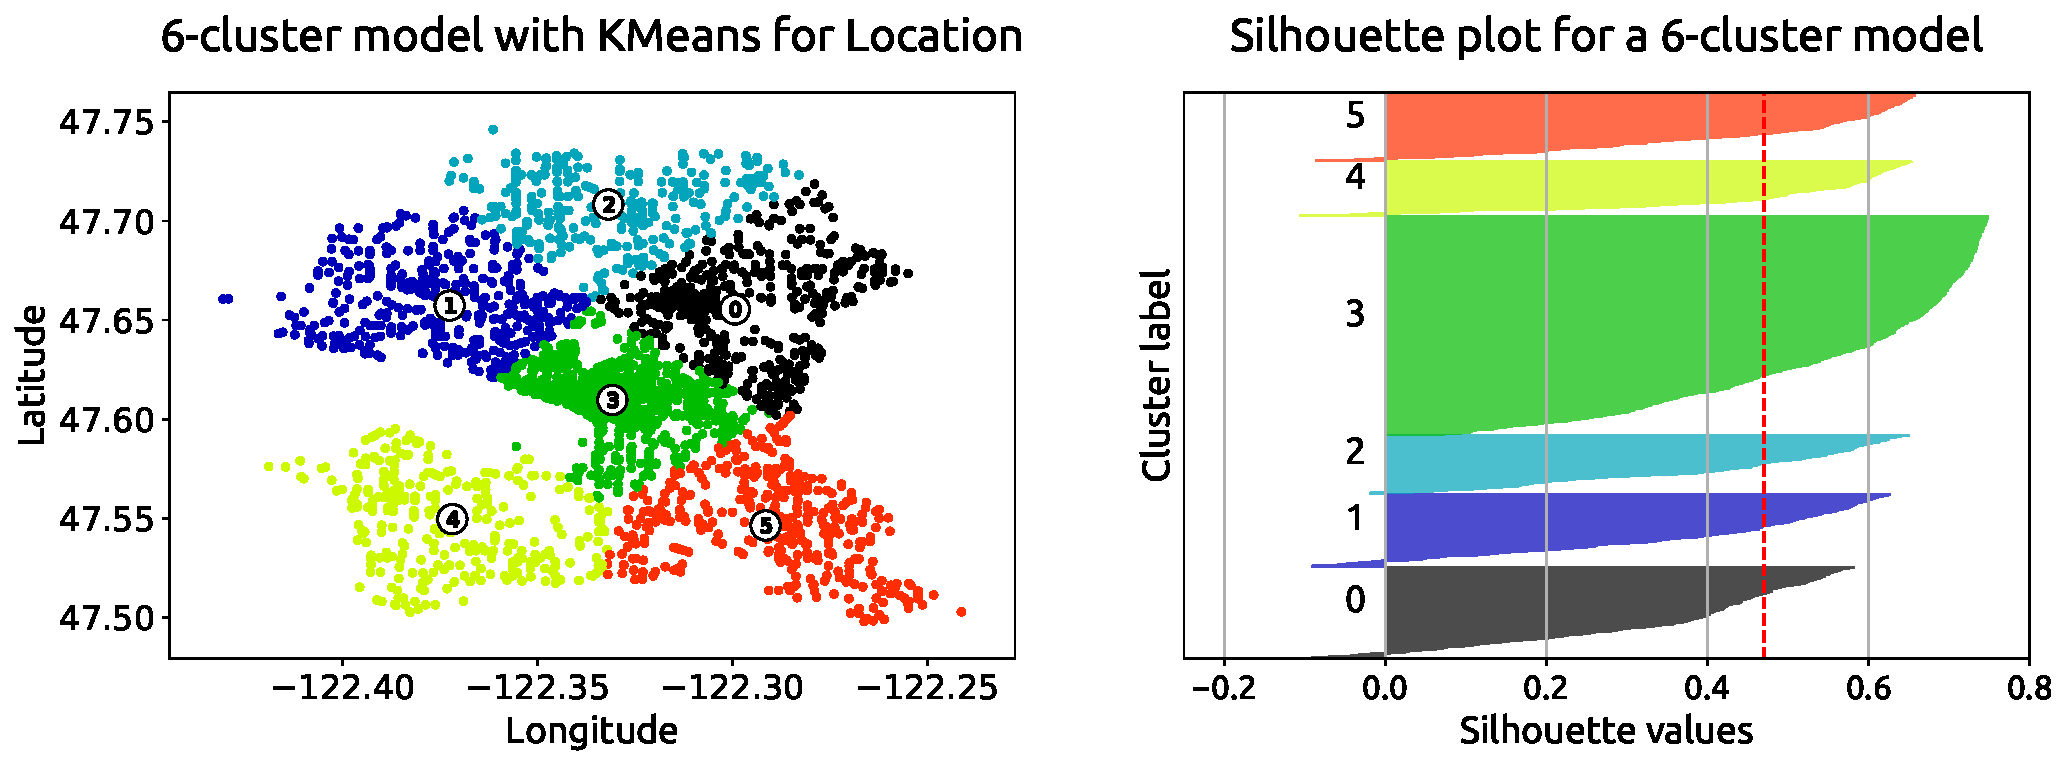
\includegraphics[scale=0.35]{figs/loc_clusfigs_6_cluster.pdf}
\end{figure}
\end{frame}

\begin{frame}{Location Clustering in other Features I}

\begin{figure}
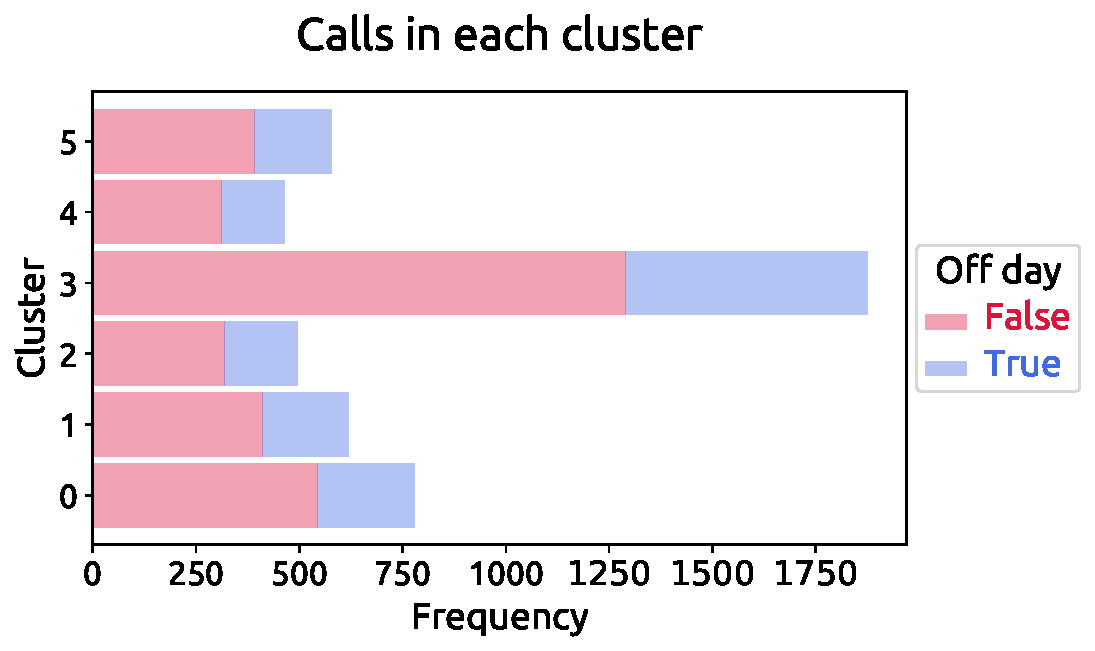
\includegraphics[scale=0.35]{figs/STORY_loc_off_days.pdf}
\hspace*{-0.9cm}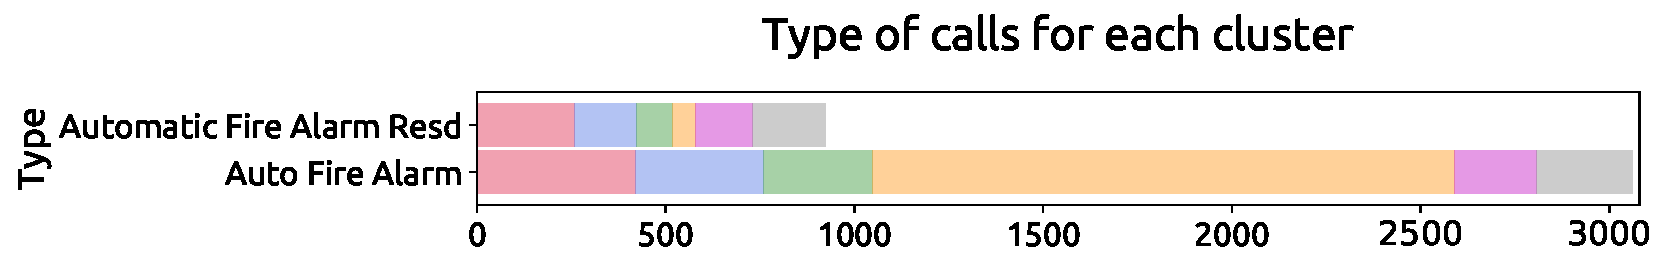
\includegraphics[scale=0.35]{figs/STORY_loc_type_1.pdf}
\end{figure}
\end{frame}

\begin{frame}{Location Clustering in other Features II}
\vspace*{-0.3cm}
\begin{figure}
\hspace*{-0.9cm}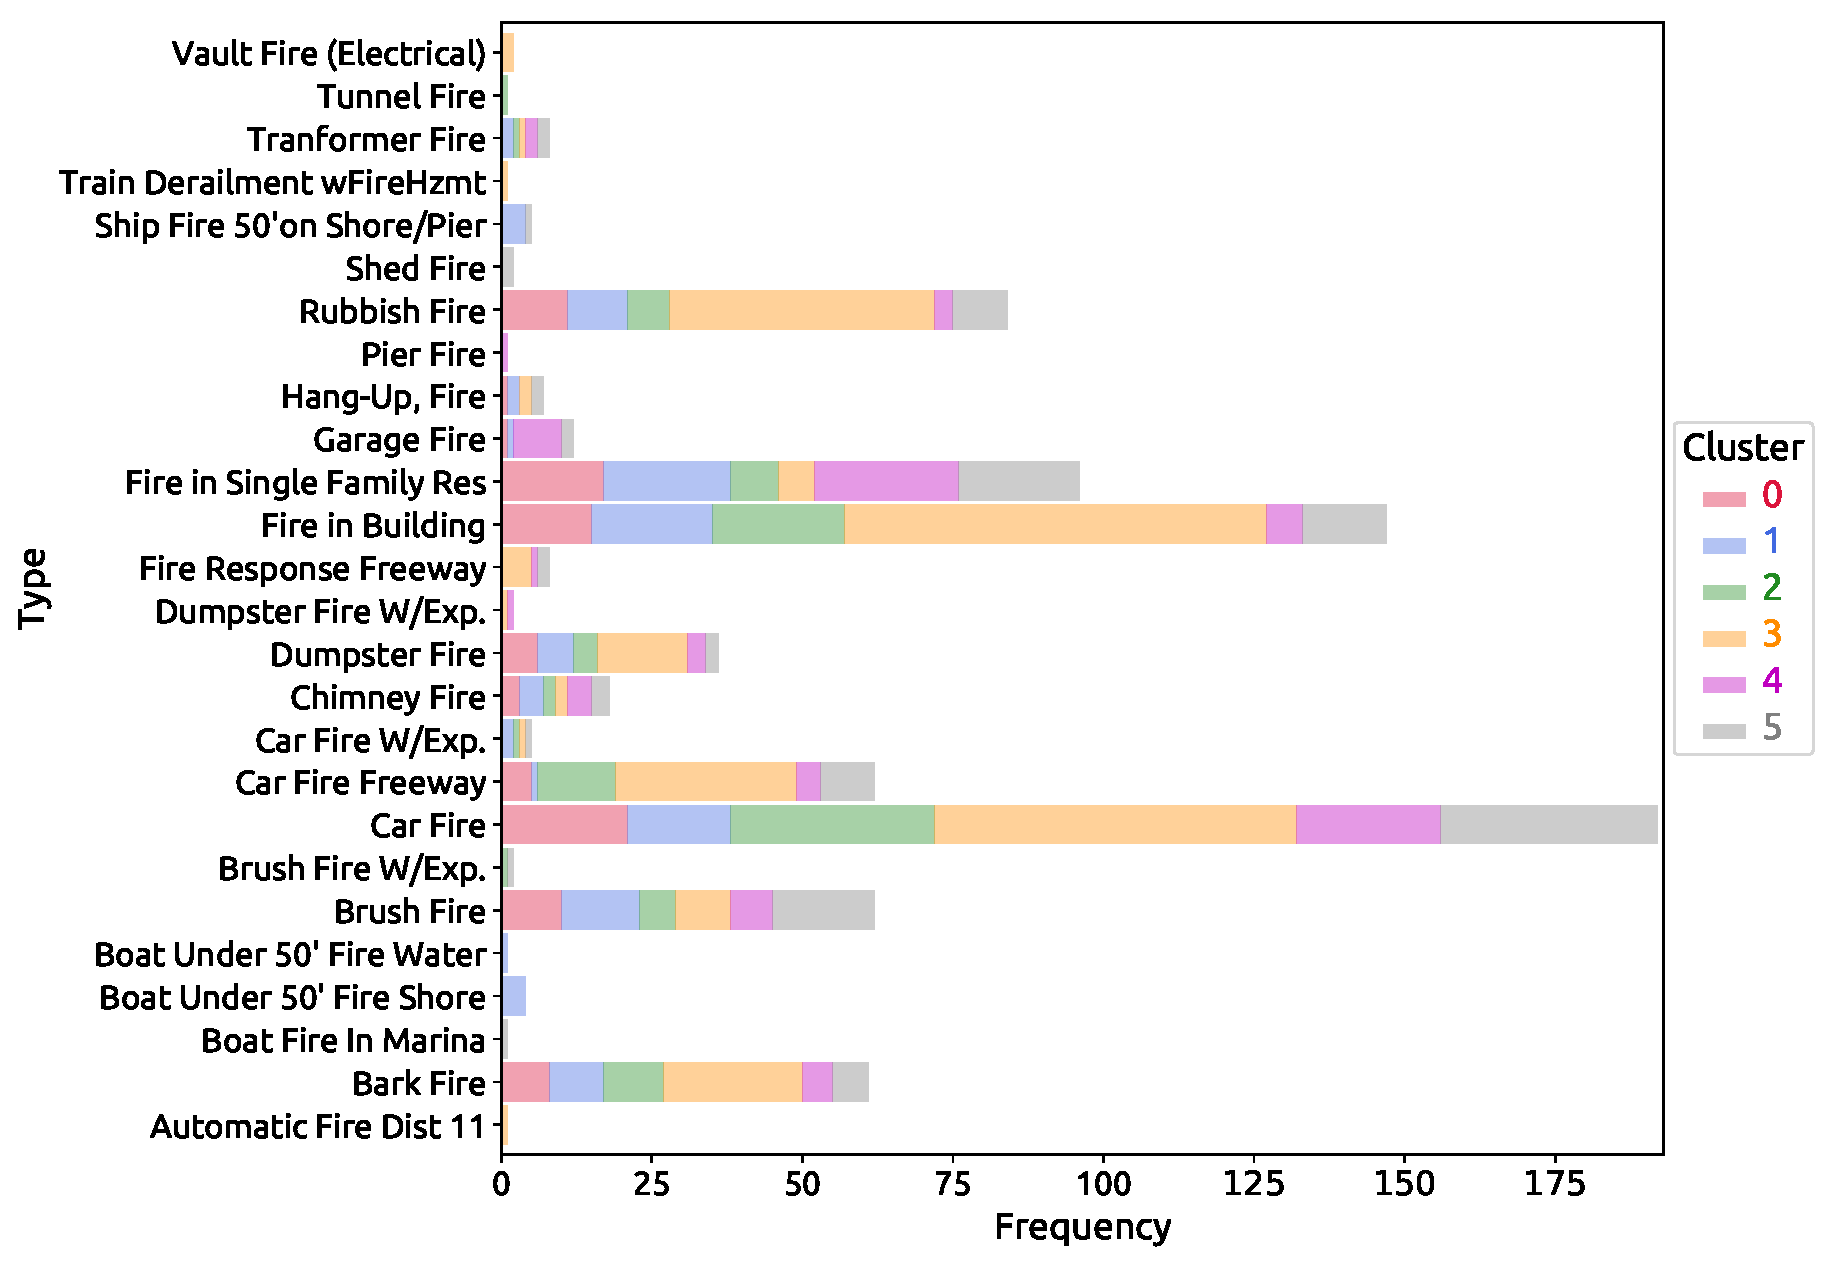
\includegraphics[scale=0.35]{figs/STORY_loc_type_2.pdf}
\end{figure}
\end{frame}

\subsection{Clustering with PCA}

\begin{frame}{Clustering with PCA: With Previous Scaling}
\begin{figure}
\hspace*{-0.9cm}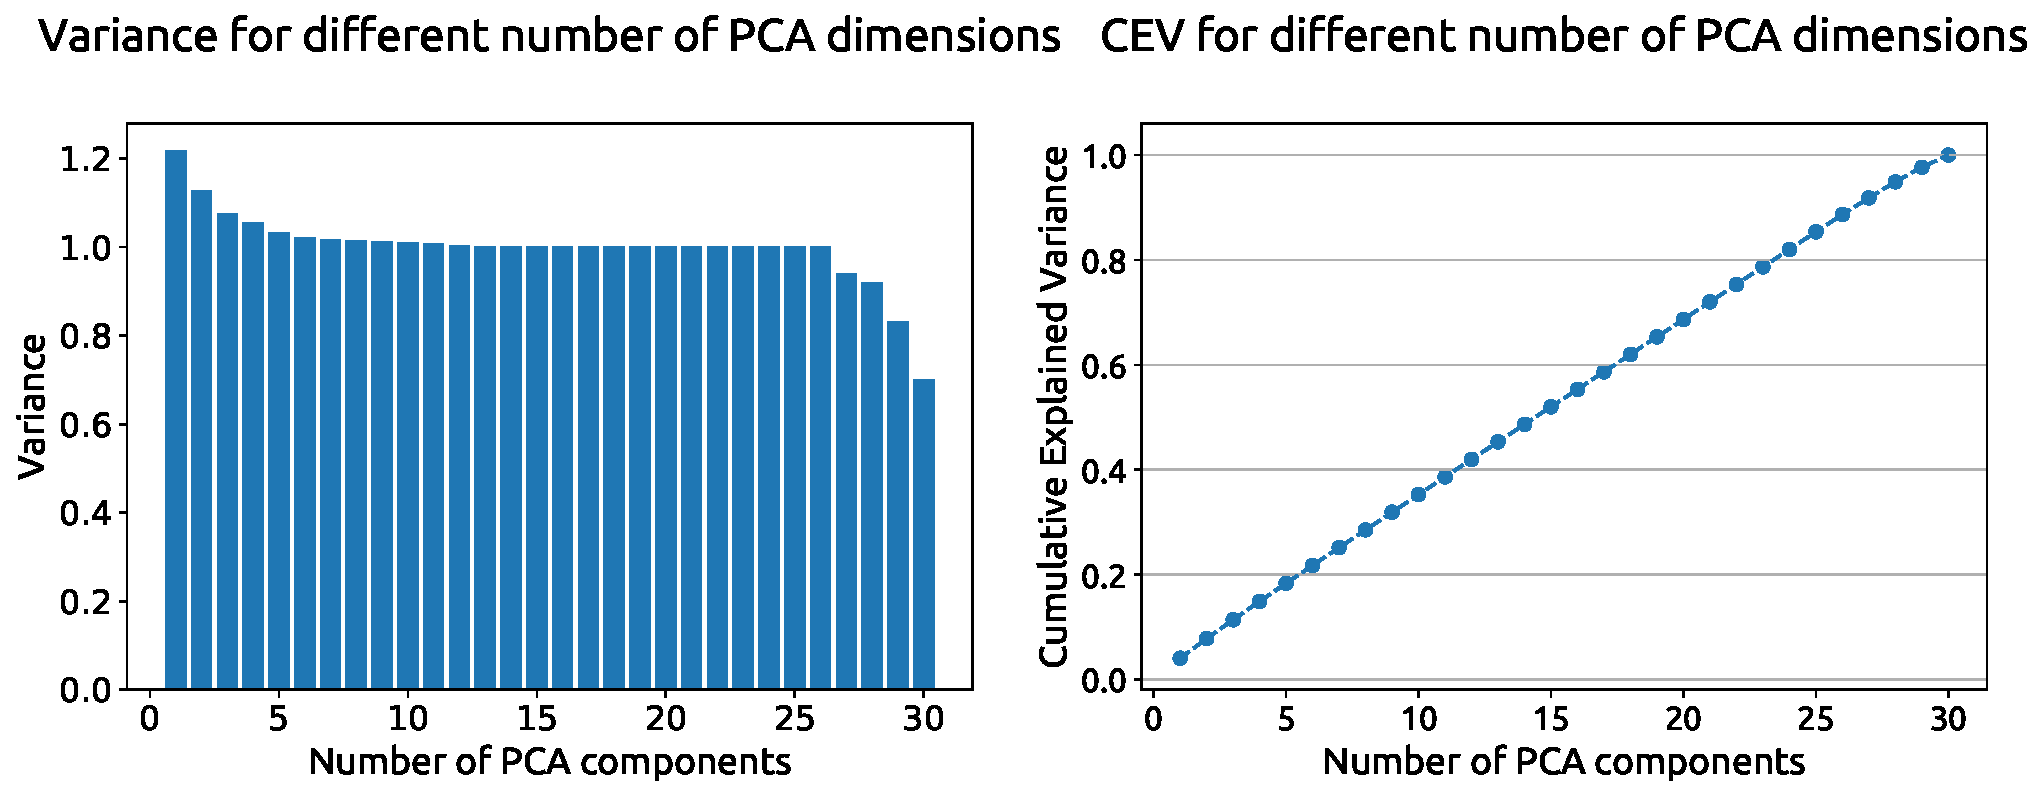
\includegraphics[scale=0.35]{figs/PCA_scaled_variance.pdf}
\end{figure}
 \end{frame}

\begin{frame}{Clustering with PCA: Without Previous Scaling}
\begin{figure}
\hspace*{-0.9cm}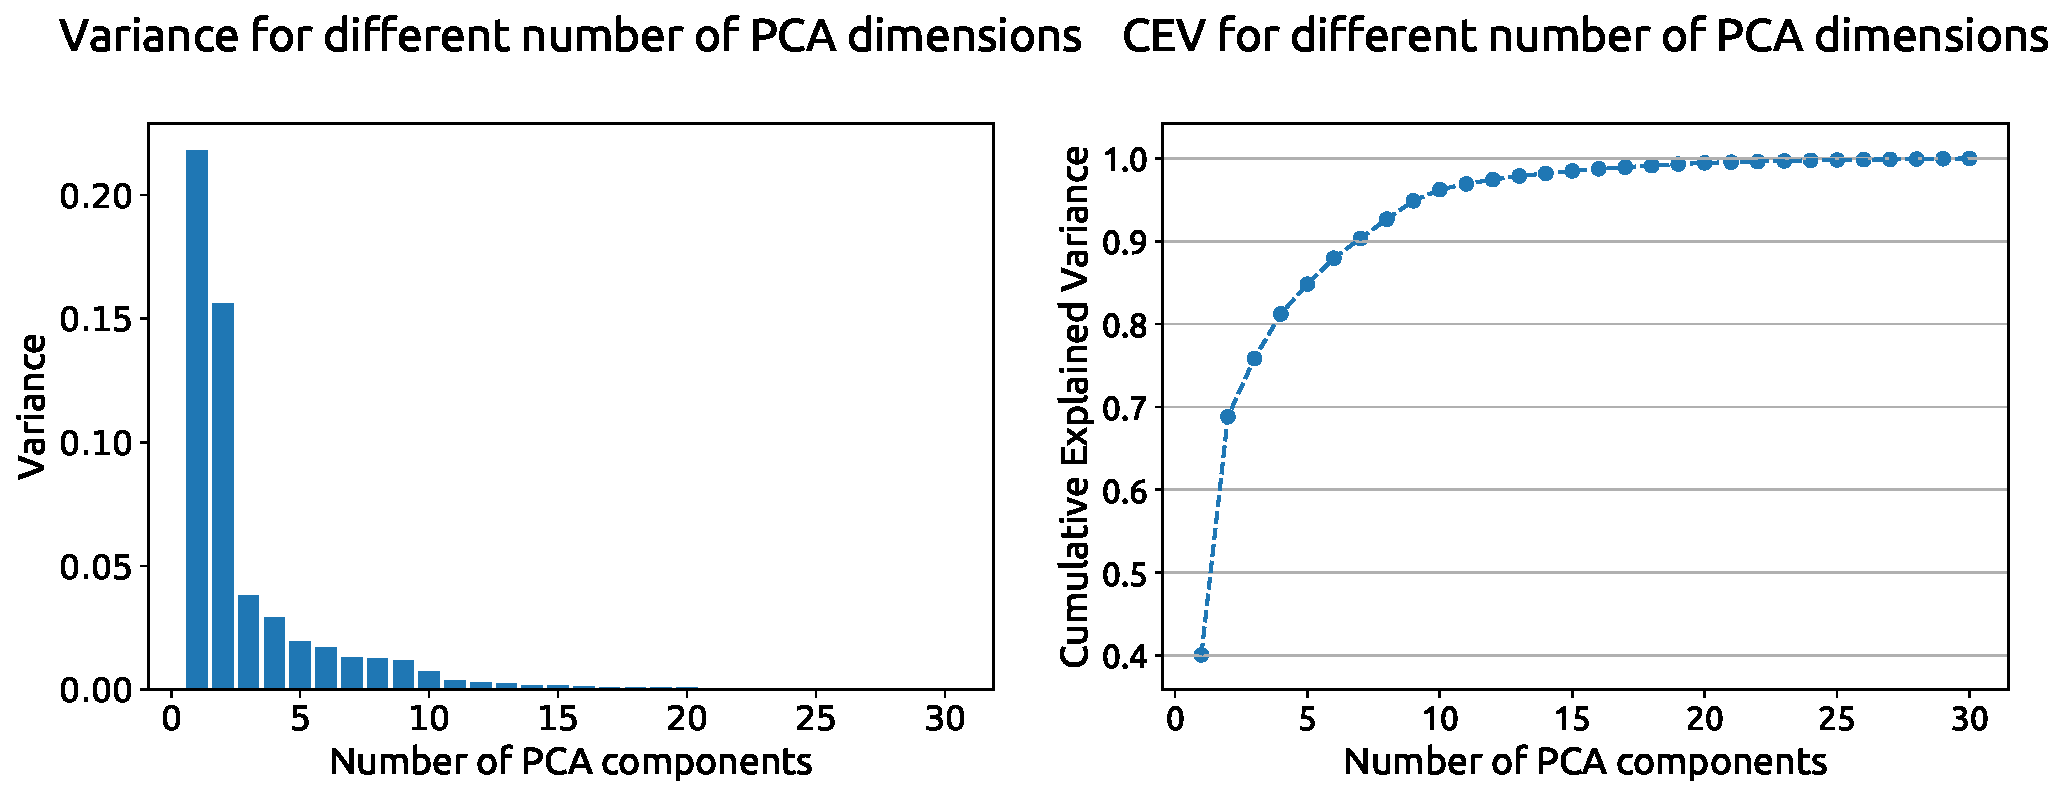
\includegraphics[scale=0.35]{figs/PCA_not_scaled_variance.pdf}
\end{figure}
 \end{frame}

\begin{frame}{Clustering with PCA: 2D and 3D}
\begin{figure}
\hspace*{-0.9cm}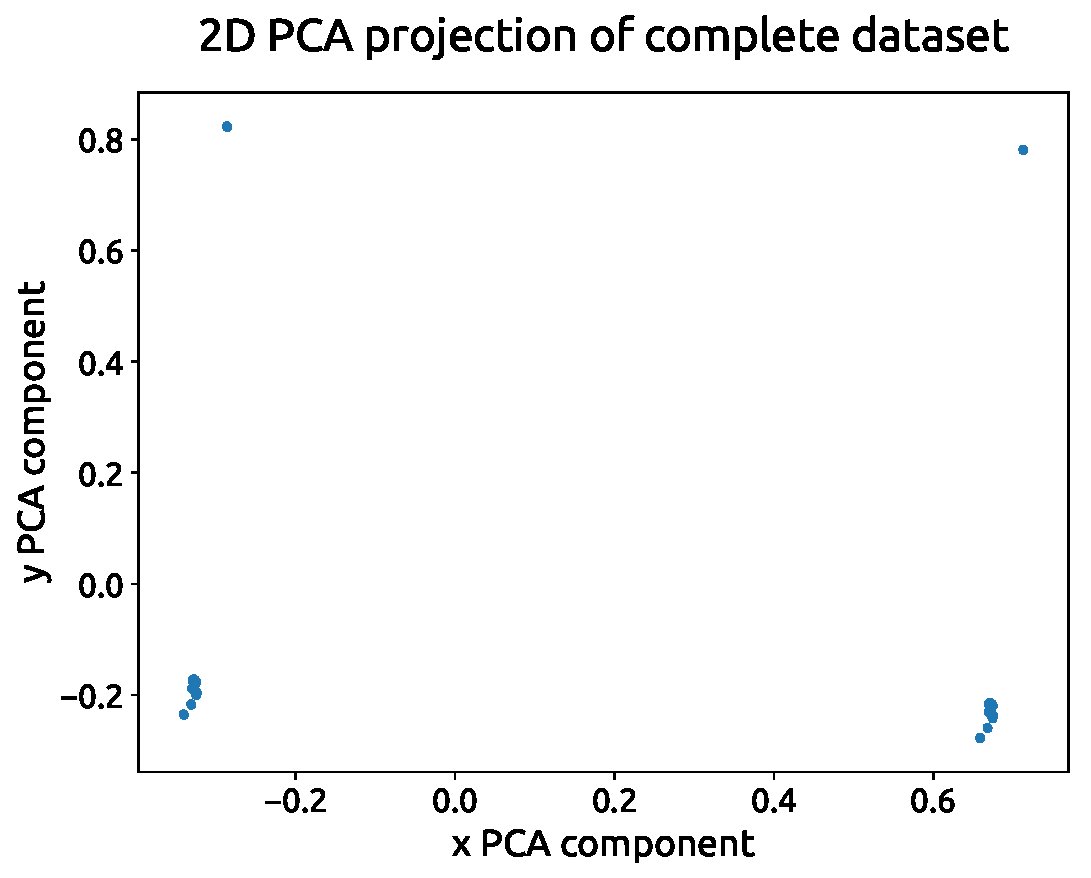
\includegraphics[width=0.54 \textwidth]{figs/PCA_2D_data.pdf}
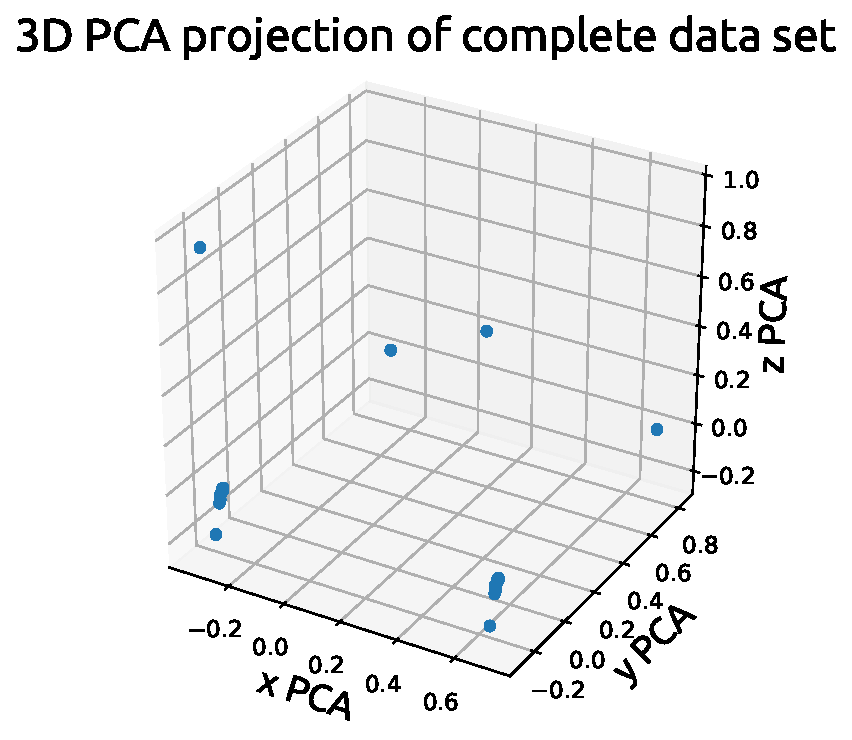
\includegraphics[width=0.45 \textwidth]{figs/PCA_3D_data.pdf}
\end{figure}
 \end{frame}


\subsection{Clustering without PCA}


\begin{frame}{Clustering without PCA: Inertia and average silhouette}
\begin{figure}
\hspace*{-0.9cm}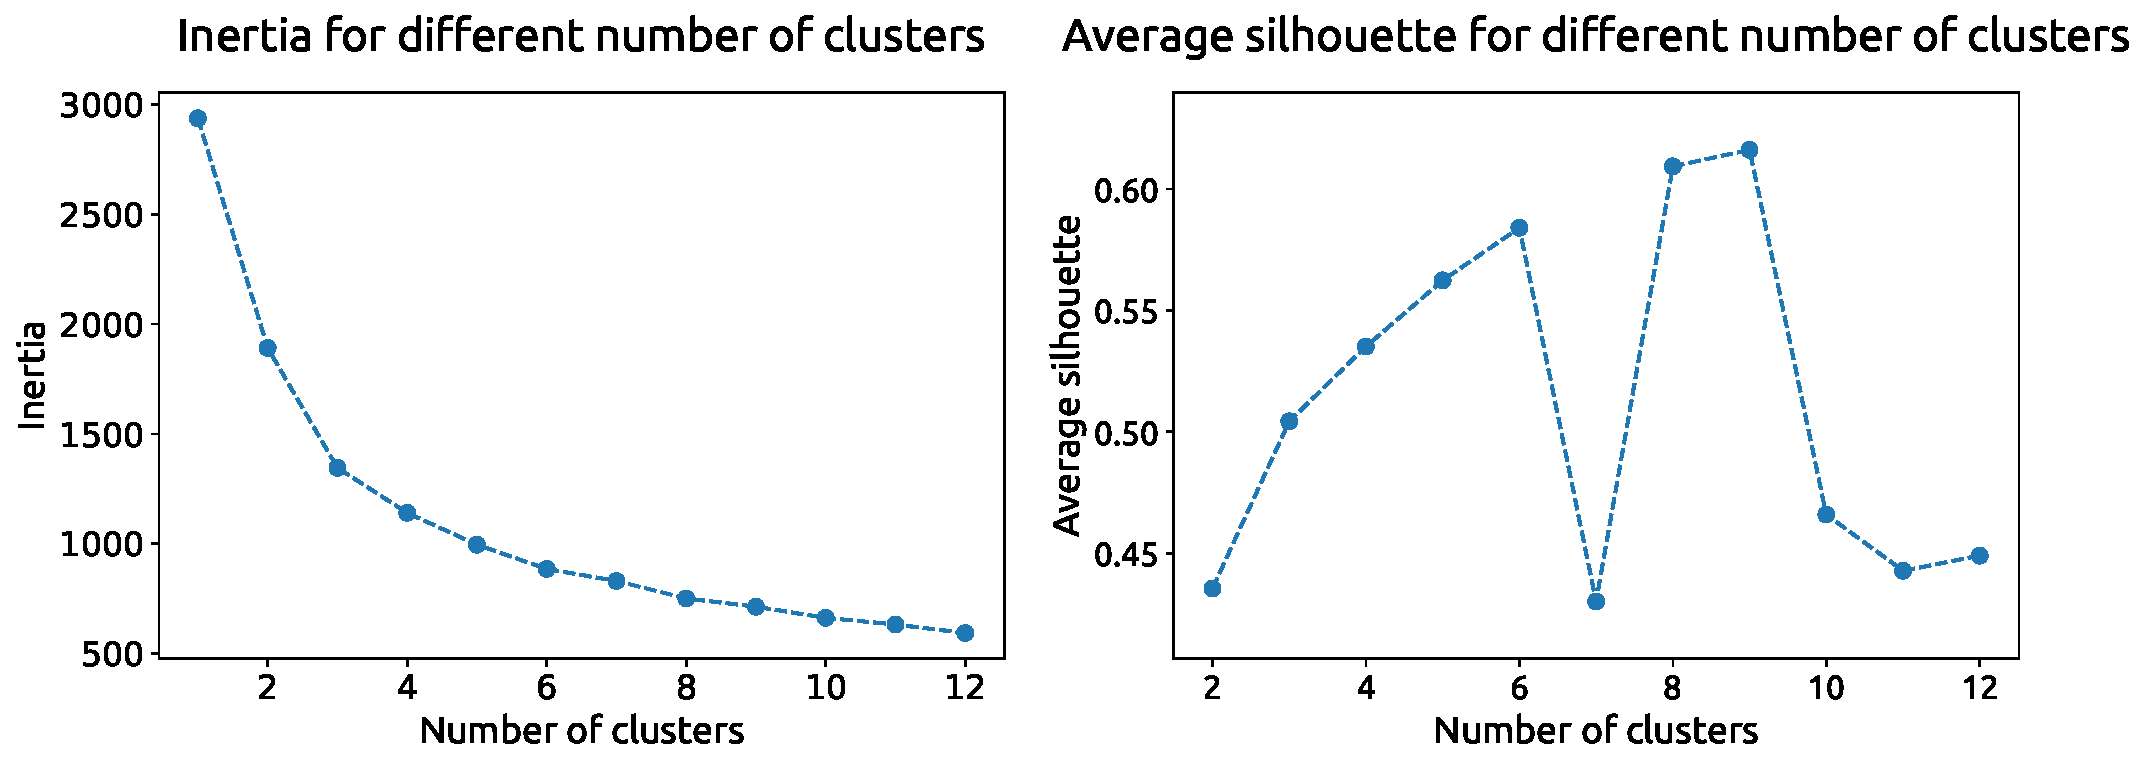
\includegraphics[scale=0.35]{figs/NO_PCA_parfigs_1.pdf}
\end{figure}
 \end{frame}

\begin{frame}{Clustering without PCA: Gap and Gap criterium}
\begin{figure}
\hspace*{-0.9cm}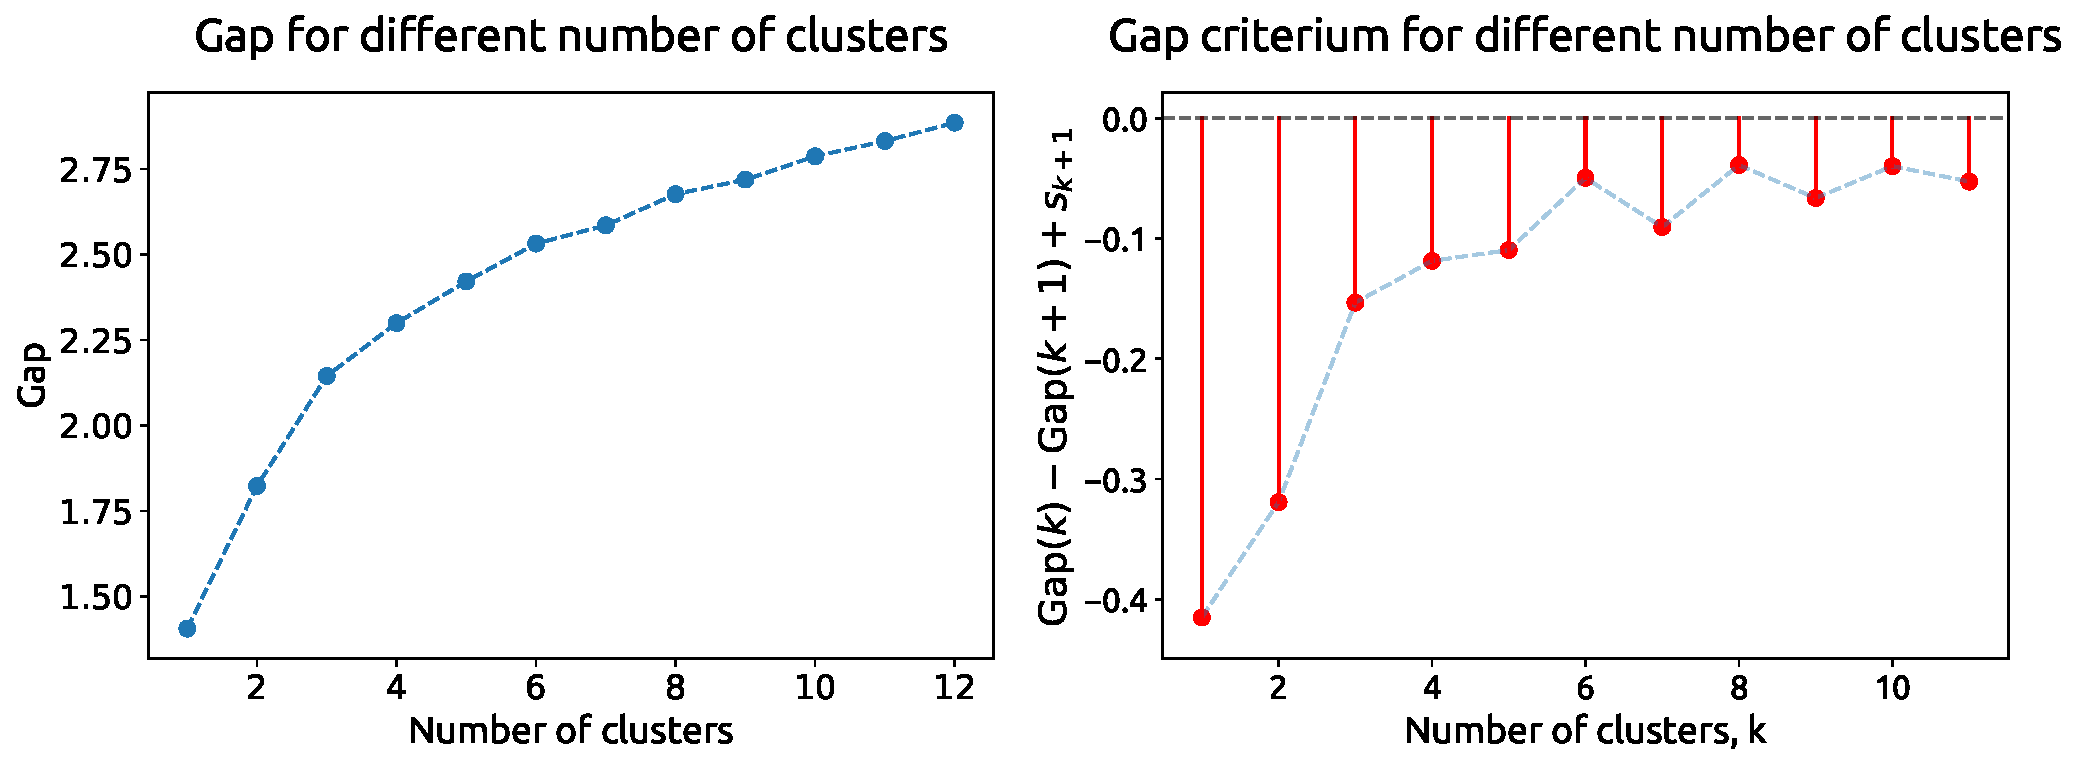
\includegraphics[scale=0.35]{figs/NO_PCA_parfigs_2.pdf}
\end{figure}

\end{frame}


\begin{frame}{Clustering without PCA: Silhouette Plot}
\begin{figure}
\hspace*{-0.9cm}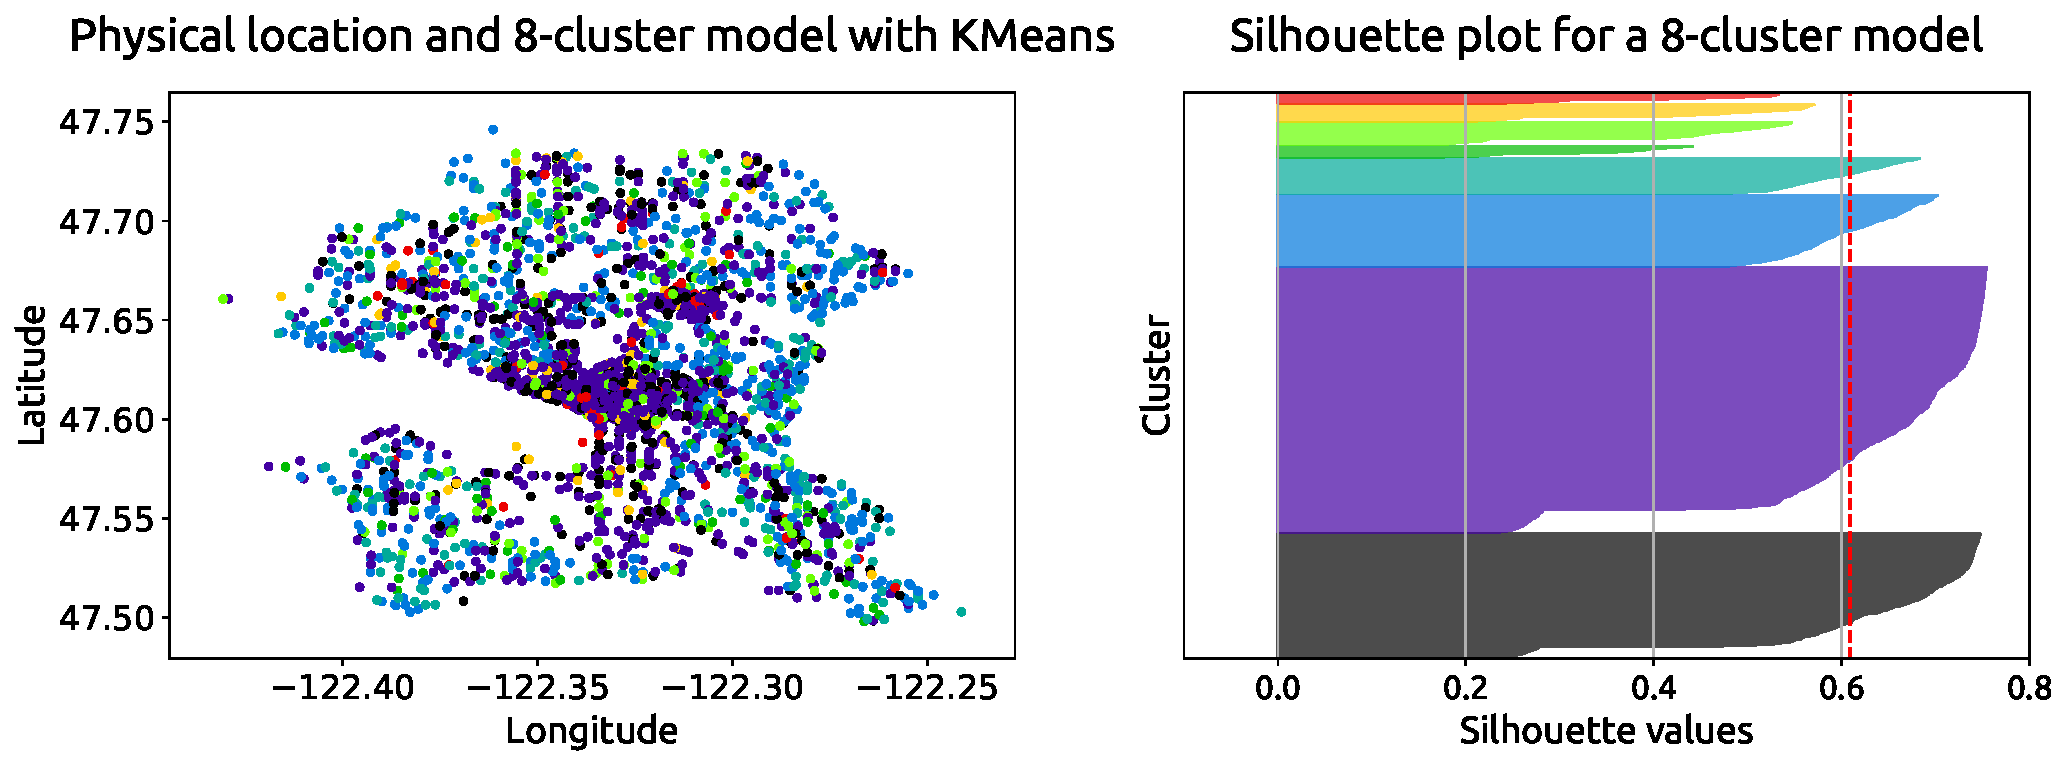
\includegraphics[scale=0.35]{figs/NO_PCA_clusfigs_8_cluster.pdf}
\end{figure}
\end{frame}

\begin{frame}{Clustering without PCA in other Features I}

\begin{figure}
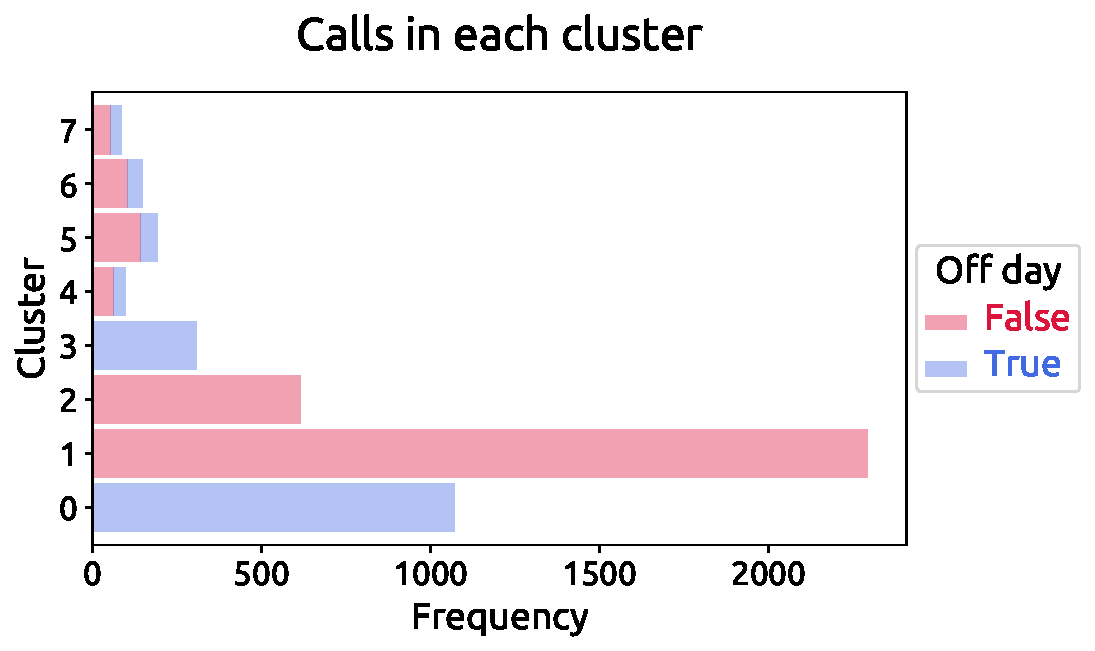
\includegraphics[scale=0.35]{figs/STORY_NO_PCA_off_days.pdf}
\hspace*{-0.9cm}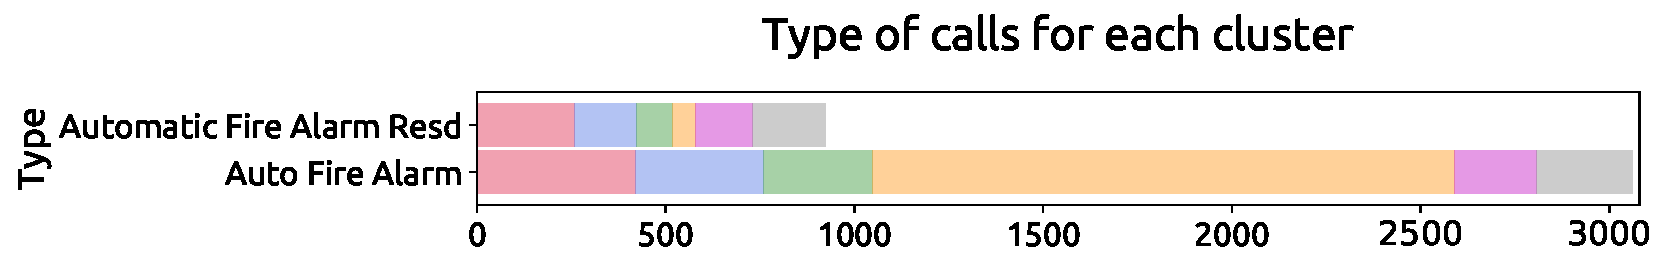
\includegraphics[scale=0.35]{figs/STORY_loc_type_1.pdf}
\end{figure}
\end{frame}

\begin{frame}{Clustering without PCA in other Features II}
\vspace*{-0.3cm}
\begin{figure}
\hspace*{-0.9cm}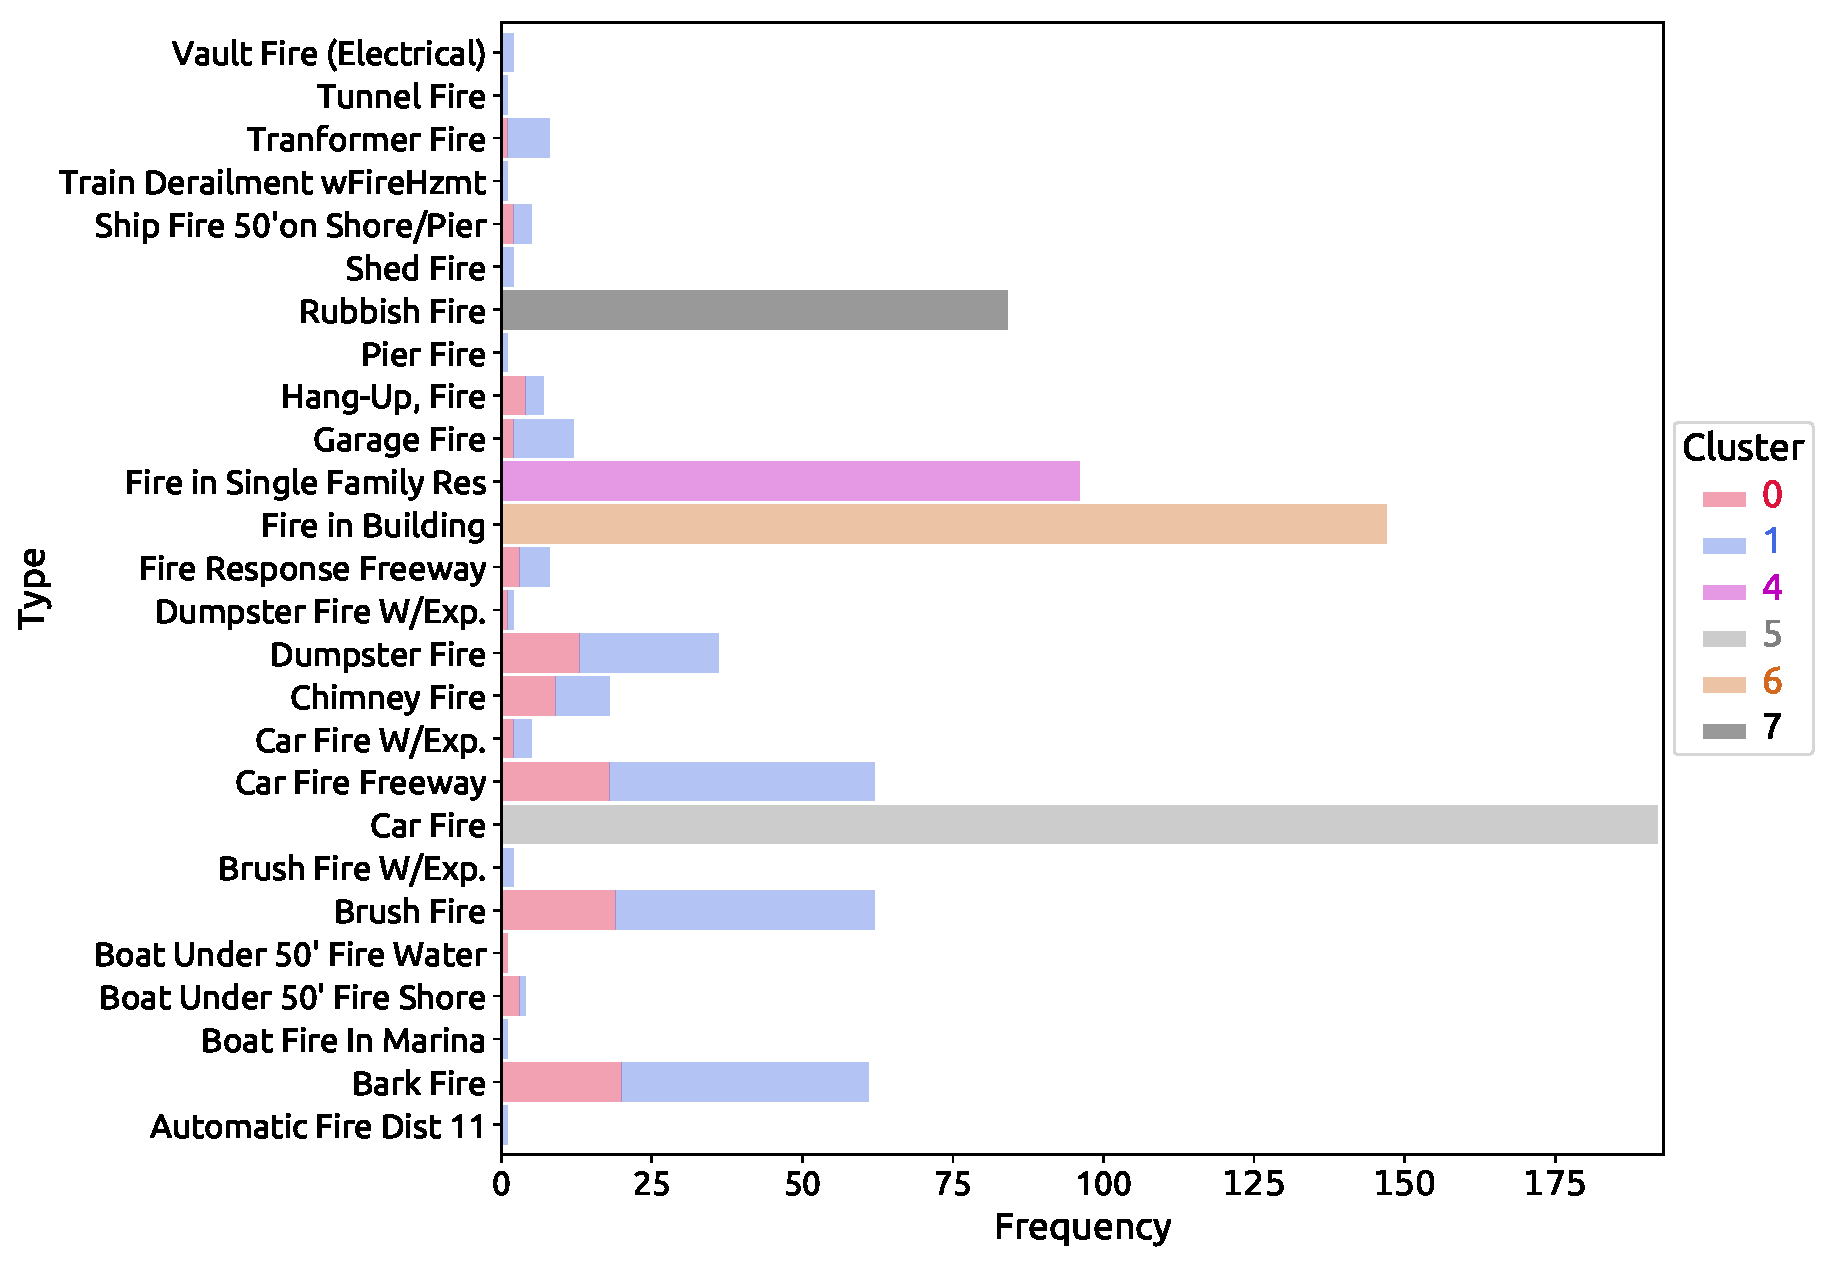
\includegraphics[scale=0.35]{figs/STORY_NO_PCA_type_2.pdf}
\end{figure}
\end{frame}

\section{Concluding Remarks}

\begin{frame}{Concluding Remarks I}
\begin{itemize}
\large
\item We found no indication that rain accumulations and the number of fire 911 calls are correlated.

\item Most of fire emergency calls happen during night time, which seems to reinforce the relevance of human factors over weather.

\item The proportion of 911 fire calls is not affected by the day being a work day or not.

\item Since 53.5\% of the fire emergencies happen in central Seattle, we should study the correlation between 911 fire calls and population density.
\end{itemize}
\end{frame}


\begin{frame}{Concluding Remarks II}
\begin{itemize}
\large
\item We obtained a data-based approach to the sectorization of the city in accordance to the number of fire emergency calls.

\item Automatic fire alarms are the most significant cause of 911 responses, even after removing false alarm calls.

\item Car fires contribute substantially in these events and Central followed by North Seattle are a priority in the amount of emergencies.

\item Policies can be focused on fires related to urban activity, specially in highly populated regions of the city, as well as night time events and on better observance of waste disposal.
\end{itemize}
\end{frame}

\begin{frame}[allowframebreaks]
\frametitle{References}
\bibliography{references}
\bibliographystyle{plain}
\end{frame}


\end{document}
